\documentclass[main]{subfiles}


\definecolor{myblue}{RGB}{0, 68, 136}
\definecolor{myred}{RGB}{187, 85, 102}
\definecolor{myyellow}{RGB}{153, 119, 0}


\definecolor{indigo}{rgb}{0.2, 0.0, 0.45}
\definecolor{indigobg}{rgb}{0.9, 0.8, 1}

\definecolor{fig2_yellow}{HTML}{FFB946}
\definecolor{Dandelion}{HTML}{FDBC42}

\definecolor{fig2_blue}{HTML}{4D9EEB}
\definecolor{Cerulean}{HTML}{00A2E3}

\definecolor{fig2_green}{HTML}{73C45D}
\definecolor{Green}{HTML}{00A64F}

\definecolor{fig2_purple}{HTML}{9E6CB3}
\definecolor{DarkOrchid}{HTML}{A4538A}

\title[AutoML: NAS]{Neural Architecture Search}
\subtitle{Beyond Simple Search Spaces}
\author[Jovita Lukasik]{Jovita Lukasik}
\date{}

\titlebackground*{images/AutoML_NAS}

%\institute{}
%\date{}

\begin{document}

	\maketitle

%----------------------------------------------------------------------
\begin{frame}{Motivation}
\begin{itemize}
    \item Existing NAS methods have achieved impressive results — but mostly on \alert{narrow, handcrafted search spaces}
    \item Studies show that on many benchmarks, \textbf{random search performs on par} with sophisticated NAS algorithms~\liturl{Yu et al. 2020}{https://openreview.net/pdf?id=H1loF2NFwr}
    \item This raises a fundamental question: are we searching in the \alert{right spaces}?
\end{itemize}
\pause
\vspace{0.5em}
\begin{colorblock}[black]{sintefgrey}{Key Question}
How can we design \textbf{more expressive search spaces} that enable NAS to discover genuinely novel architectures?
\end{colorblock}
\end{frame}

\begin{frame}{Issues with Current Search Spaces}
\begin{center}
    
    \textit{``On average, the state-of-the-art NAS algorithms perform similarly to the random policy''} \\[2em]
\hfill by \liturl{Yu et al. 2020}{https://openreview.net/pdf?id=H1loF2NFwr} 
\end{center}
\begin{itemize}
    \item Most existing search spaces are limited and narrow with many high-performing architectures 
    \item Most search spaces are based on ConvNets
\end{itemize}

\end{frame}

\begin{frame}{AutoML-Zero \liturl{Real et al. 2020}{https://arxiv.org/pdf/2003.03384}}
Larger Search Space $\rightarrow$ Search Strategy is important
\begin{itemize}
    \item It is hard to find good architectures in larger search spaces
\end{itemize}

    \begin{figure}
        \centering
        
\includegraphics[width=0.5\linewidth]{07_NAS/images/07/relative_difficulty.pdf}
        \caption{AutoML-Zero \liturl{Real et al. 2020}{https://arxiv.org/pdf/2003.03384}}
    \end{figure}
\end{frame}

\begin{frame}{AutoML-Zero \liturl{Real et al. 2020}{https://arxiv.org/pdf/2003.03384}}

    \begin{figure}
        \centering
        
\includegraphics[width=0.6\linewidth]{07_NAS/images/07/AutoML_zero.png}
        \caption{AutoML-Zero \liturl{Real et al. 2020}{https://arxiv.org/pdf/2003.03384}}
    \end{figure}
    
\end{frame}
\begin{frame}{Expressive Search Space}
AutoML-Zero: First step towards large, expressive search space, but requires a huge time budget, to find a simple network

We want a search space,
\begin{itemize}
    \item which is expressive enough to contain diverse architectures
    \item which is not too large that search slows down too much 
    
\end{itemize}
    
\end{frame}

\begin{frame}{Architectures as Composition of Functions}
\begin{center}

\end{center}
% \onslide<1-2>
\begin{equation*}\label{eq:anae_example}
        \texttt{Sequential}(\texttt{Residual}(\texttt{conv},\;\texttt{id},\;\texttt{conv}),
        \texttt{Residual}(\texttt{conv},\;\texttt{id},\;\texttt{conv}),
        \texttt{linear}) \quad ,
\end{equation*}

% \onslide<2-3>
\tikzset{every picture/.style={line width=0.75pt}} %set default line width to 0.75pt        
\begin{center}
    
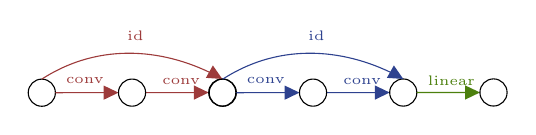
\begin{tikzpicture}[x=0.75pt,y=0.75pt,yscale=-1,xscale=1, scale=0.8]
%uncomment if require: \path (0,66); %set diagram left start at 0, and has height of 66

%Shape: Circle [id:dp49584175205407666] 
\draw   (1.79,43.83) .. controls (1.79,39.31) and (5.45,35.65) .. (9.96,35.65) .. controls (14.48,35.65) and (18.14,39.31) .. (18.14,43.83) .. controls (18.14,48.34) and (14.48,52) .. (9.96,52) .. controls (5.45,52) and (1.79,48.34) .. (1.79,43.83) -- cycle ;
%Straight Lines [id:da8268391580818041] 
\draw [color={rgb, 255:red, 157; green, 59; blue, 59 }  ,draw opacity=1 ]   (18.14,43.83) -- (49.45,43.79) -- (53.14,43.78) ;
\draw [shift={(56.14,43.78)}, rotate = 179.93] [fill={rgb, 255:red, 157; green, 59; blue, 59 }  ,fill opacity=1 ][line width=0.08]  [draw opacity=0] (8.93,-4.29) -- (0,0) -- (8.93,4.29) -- cycle    ;
%Straight Lines [id:da48759814276871993] 
\draw [color={rgb, 255:red, 157; green, 59; blue, 59 }  ,draw opacity=1 ]   (72.48,43.78) -- (103.8,43.74) -- (107.48,43.74) ;
\draw [shift={(110.48,43.73)}, rotate = 179.93] [fill={rgb, 255:red, 157; green, 59; blue, 59 }  ,fill opacity=1 ][line width=0.08]  [draw opacity=0] (8.93,-4.29) -- (0,0) -- (8.93,4.29) -- cycle    ;
%Shape: Circle [id:dp9840360565179291] 
\draw   (56.14,43.78) .. controls (56.14,39.27) and (59.8,35.61) .. (64.31,35.61) .. controls (68.82,35.61) and (72.48,39.27) .. (72.48,43.78) .. controls (72.48,48.29) and (68.82,51.95) .. (64.31,51.95) .. controls (59.8,51.95) and (56.14,48.29) .. (56.14,43.78) -- cycle ;
%Shape: Circle [id:dp6896881129107634] 
\draw   (110.48,43.73) .. controls (110.48,39.22) and (114.14,35.56) .. (118.66,35.56) .. controls (123.17,35.56) and (126.83,39.22) .. (126.83,43.73) .. controls (126.83,48.25) and (123.17,51.91) .. (118.66,51.91) .. controls (114.14,51.91) and (110.48,48.25) .. (110.48,43.73) -- cycle ;
%Curve Lines [id:da45397432309361974] 
\draw [color={rgb, 255:red, 157; green, 59; blue, 59 }  ,draw opacity=1 ]   (9.96,35.65) .. controls (45.72,12.56) and (85.59,17.69) .. (116.31,34.26) ;
\draw [shift={(118.66,35.56)}, rotate = 209.56] [fill={rgb, 255:red, 157; green, 59; blue, 59 }  ,fill opacity=1 ][line width=0.08]  [draw opacity=0] (8.93,-4.29) -- (0,0) -- (8.93,4.29) -- cycle    ;
%Shape: Circle [id:dp6270373103109923] 
\draw   (110.79,43.83) .. controls (110.79,39.31) and (114.45,35.65) .. (118.96,35.65) .. controls (123.48,35.65) and (127.14,39.31) .. (127.14,43.83) .. controls (127.14,48.34) and (123.48,52) .. (118.96,52) .. controls (114.45,52) and (110.79,48.34) .. (110.79,43.83) -- cycle ;
%Straight Lines [id:da28650876217853805] 
\draw [color={rgb, 255:red, 46; green, 66; blue, 143 }  ,draw opacity=1 ]   (127.14,43.83) -- (158.45,43.79) -- (162.14,43.78) ;
\draw [shift={(165.14,43.78)}, rotate = 179.93] [fill={rgb, 255:red, 46; green, 66; blue, 143 }  ,fill opacity=1 ][line width=0.08]  [draw opacity=0] (8.93,-4.29) -- (0,0) -- (8.93,4.29) -- cycle    ;
%Straight Lines [id:da9639159191291868] 
\draw [color={rgb, 255:red, 46; green, 66; blue, 143 }  ,draw opacity=1 ]   (181.48,43.78) -- (212.8,43.74) -- (216.48,43.74) ;
\draw [shift={(219.48,43.73)}, rotate = 179.93] [fill={rgb, 255:red, 46; green, 66; blue, 143 }  ,fill opacity=1 ][line width=0.08]  [draw opacity=0] (8.93,-4.29) -- (0,0) -- (8.93,4.29) -- cycle    ;
%Shape: Circle [id:dp8745570630773656] 
\draw   (165.14,43.78) .. controls (165.14,39.27) and (168.8,35.61) .. (173.31,35.61) .. controls (177.82,35.61) and (181.48,39.27) .. (181.48,43.78) .. controls (181.48,48.29) and (177.82,51.95) .. (173.31,51.95) .. controls (168.8,51.95) and (165.14,48.29) .. (165.14,43.78) -- cycle ;
%Shape: Circle [id:dp8652422385738179] 
\draw   (219.48,43.73) .. controls (219.48,39.22) and (223.14,35.56) .. (227.66,35.56) .. controls (232.17,35.56) and (235.83,39.22) .. (235.83,43.73) .. controls (235.83,48.25) and (232.17,51.91) .. (227.66,51.91) .. controls (223.14,51.91) and (219.48,48.25) .. (219.48,43.73) -- cycle ;
%Curve Lines [id:da38214051995450027] 
\draw [color={rgb, 255:red, 46; green, 66; blue, 143 }  ,draw opacity=1 ]   (118.96,35.65) .. controls (154.72,12.56) and (194.59,17.69) .. (225.31,34.26) ;
\draw [shift={(227.66,35.56)}, rotate = 209.56] [fill={rgb, 255:red, 46; green, 66; blue, 143 }  ,fill opacity=1 ][line width=0.08]  [draw opacity=0] (8.93,-4.29) -- (0,0) -- (8.93,4.29) -- cycle    ;
%Straight Lines [id:da2966608138594343] 
\draw [color={rgb, 255:red, 76; green, 128; blue, 14 }  ,draw opacity=1 ]   (235.83,43.73) -- (267.15,43.7) -- (270.83,43.69) ;
\draw [shift={(273.83,43.69)}, rotate = 179.93] [fill={rgb, 255:red, 76; green, 128; blue, 14 }  ,fill opacity=1 ][line width=0.08]  [draw opacity=0] (8.93,-4.29) -- (0,0) -- (8.93,4.29) -- cycle    ;
%Shape: Circle [id:dp9308784378852808] 
\draw   (273.83,43.69) .. controls (273.83,39.17) and (277.49,35.51) .. (282.01,35.51) .. controls (286.52,35.51) and (290.18,39.17) .. (290.18,43.69) .. controls (290.18,48.2) and (286.52,51.86) .. (282.01,51.86) .. controls (277.49,51.86) and (273.83,48.2) .. (273.83,43.69) -- cycle ;

% Text Node
\draw (22.96,33) node [anchor=north west][inner sep=0.75pt]  [font=\tiny,color={rgb, 255:red, 157; green, 59; blue, 59 }  ,opacity=1 ] [align=left] {conv};
% Text Node
\draw (80.96,34) node [anchor=north west][inner sep=0.75pt]  [font=\tiny,color={rgb, 255:red, 157; green, 59; blue, 59 }  ,opacity=1 ] [align=left] {conv};
% Text Node
\draw (59.96,5) node [anchor=north west][inner sep=0.75pt]  [font=\tiny,color={rgb, 255:red, 157; green, 59; blue, 59 }  ,opacity=1 ] [align=left] {id};
% Text Node
\draw (131.96,33) node [anchor=north west][inner sep=0.75pt]  [font=\tiny,color={rgb, 255:red, 46; green, 66; blue, 143 }  ,opacity=1 ] [align=left] {conv};
% Text Node
\draw (189.96,34) node [anchor=north west][inner sep=0.75pt]  [font=\tiny,color={rgb, 255:red, 46; green, 66; blue, 143 }  ,opacity=1 ] [align=left] {conv};
% Text Node
\draw (168.96,5) node [anchor=north west][inner sep=0.75pt]  [font=\tiny,color={rgb, 255:red, 46; green, 66; blue, 143 }  ,opacity=1 ] [align=left] {id};
% Text Node
\draw (240.96,32) node [anchor=north west][inner sep=0.75pt]  [font=\tiny,color={rgb, 255:red, 76; green, 128; blue, 14 }  ,opacity=1 ] [align=left] {linear};
\end{tikzpicture}
\end{center}
% \onslide<3>
\begin{columns}
\begin{column}{0.5\textwidth}
    Sequential(\newline
    \hspace*{.1\textwidth} \textcolor[HTML]{9D3B3B}{Residual(conv,id,conv)}, \newline
    \hspace*{.1\textwidth}  \textcolor[HTML]{2E428F}{Residual(conv,id,conv)}, \newline
    \hspace*{.1\textwidth}  \textcolor[HTML]{4C800E}{linear} \newline
    )
\end{column}
\begin{column}{0.5\textwidth}


\tikzset{every picture/.style={line width=0.75pt}} %set default line width to 0.75pt        

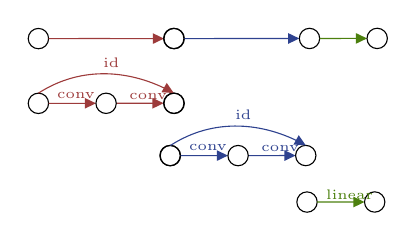
\begin{tikzpicture}[x=0.75pt,y=0.75pt,yscale=-1,xscale=1, scale=0.6]
%uncomment if require: \path (0,300); %set diagram left start at 0, and has height of 300

%Shape: Circle [id:dp20940861447111103] 
\draw   (73.79,100.83) .. controls (73.79,96.31) and (77.45,92.65) .. (81.96,92.65) .. controls (86.48,92.65) and (90.14,96.31) .. (90.14,100.83) .. controls (90.14,105.34) and (86.48,109) .. (81.96,109) .. controls (77.45,109) and (73.79,105.34) .. (73.79,100.83) -- cycle ;
%Straight Lines [id:da6677619518100352] 
\draw [color={rgb, 255:red, 157; green, 59; blue, 59 }  ,draw opacity=1 ]   (90.14,100.83) -- (121.45,100.79) -- (179.79,100.82) ;
\draw [shift={(182.79,100.83)}, rotate = 180.04] [fill={rgb, 255:red, 157; green, 59; blue, 59 }  ,fill opacity=1 ][line width=0.08]  [draw opacity=0] (8.93,-4.29) -- (0,0) -- (8.93,4.29) -- cycle    ;
%Shape: Circle [id:dp6006183449981286] 
\draw   (182.48,100.73) .. controls (182.48,96.22) and (186.14,92.56) .. (190.66,92.56) .. controls (195.17,92.56) and (198.83,96.22) .. (198.83,100.73) .. controls (198.83,105.25) and (195.17,108.91) .. (190.66,108.91) .. controls (186.14,108.91) and (182.48,105.25) .. (182.48,100.73) -- cycle ;
%Shape: Circle [id:dp4210346910211946] 
\draw   (182.79,100.83) .. controls (182.79,96.31) and (186.45,92.65) .. (190.96,92.65) .. controls (195.48,92.65) and (199.14,96.31) .. (199.14,100.83) .. controls (199.14,105.34) and (195.48,109) .. (190.96,109) .. controls (186.45,109) and (182.79,105.34) .. (182.79,100.83) -- cycle ;
%Straight Lines [id:da33810450354858446] 
\draw [color={rgb, 255:red, 46; green, 66; blue, 143 }  ,draw opacity=1 ]   (199.14,100.83) -- (230.45,100.79) -- (288.48,100.74) ;
\draw [shift={(291.48,100.73)}, rotate = 179.95] [fill={rgb, 255:red, 46; green, 66; blue, 143 }  ,fill opacity=1 ][line width=0.08]  [draw opacity=0] (8.93,-4.29) -- (0,0) -- (8.93,4.29) -- cycle    ;
%Shape: Circle [id:dp24579686966366987] 
\draw   (291.48,100.73) .. controls (291.48,96.22) and (295.14,92.56) .. (299.66,92.56) .. controls (304.17,92.56) and (307.83,96.22) .. (307.83,100.73) .. controls (307.83,105.25) and (304.17,108.91) .. (299.66,108.91) .. controls (295.14,108.91) and (291.48,105.25) .. (291.48,100.73) -- cycle ;
%Straight Lines [id:da6431089119412706] 
\draw [color={rgb, 255:red, 76; green, 128; blue, 14 }  ,draw opacity=1 ]   (307.83,100.73) -- (339.15,100.7) -- (342.83,100.69) ;
\draw [shift={(345.83,100.69)}, rotate = 179.93] [fill={rgb, 255:red, 76; green, 128; blue, 14 }  ,fill opacity=1 ][line width=0.08]  [draw opacity=0] (8.93,-4.29) -- (0,0) -- (8.93,4.29) -- cycle    ;
%Shape: Circle [id:dp7313733674753292] 
\draw   (345.83,100.69) .. controls (345.83,96.17) and (349.49,92.51) .. (354.01,92.51) .. controls (358.52,92.51) and (362.18,96.17) .. (362.18,100.69) .. controls (362.18,105.2) and (358.52,108.86) .. (354.01,108.86) .. controls (349.49,108.86) and (345.83,105.2) .. (345.83,100.69) -- cycle ;
%Shape: Circle [id:dp5472204841987968] 
\draw   (73.79,152.83) .. controls (73.79,148.31) and (77.45,144.65) .. (81.96,144.65) .. controls (86.48,144.65) and (90.14,148.31) .. (90.14,152.83) .. controls (90.14,157.34) and (86.48,161) .. (81.96,161) .. controls (77.45,161) and (73.79,157.34) .. (73.79,152.83) -- cycle ;
%Straight Lines [id:da09885057162055966] 
\draw [color={rgb, 255:red, 157; green, 59; blue, 59 }  ,draw opacity=1 ]   (90.14,152.83) -- (121.45,152.79) -- (125.14,152.78) ;
\draw [shift={(128.14,152.78)}, rotate = 179.93] [fill={rgb, 255:red, 157; green, 59; blue, 59 }  ,fill opacity=1 ][line width=0.08]  [draw opacity=0] (8.93,-4.29) -- (0,0) -- (8.93,4.29) -- cycle    ;
%Straight Lines [id:da638536764580979] 
\draw [color={rgb, 255:red, 157; green, 59; blue, 59 }  ,draw opacity=1 ]   (144.48,152.78) -- (175.8,152.74) -- (179.48,152.74) ;
\draw [shift={(182.48,152.73)}, rotate = 179.93] [fill={rgb, 255:red, 157; green, 59; blue, 59 }  ,fill opacity=1 ][line width=0.08]  [draw opacity=0] (8.93,-4.29) -- (0,0) -- (8.93,4.29) -- cycle    ;
%Shape: Circle [id:dp23795362993512315] 
\draw   (128.14,152.78) .. controls (128.14,148.27) and (131.8,144.61) .. (136.31,144.61) .. controls (140.82,144.61) and (144.48,148.27) .. (144.48,152.78) .. controls (144.48,157.29) and (140.82,160.95) .. (136.31,160.95) .. controls (131.8,160.95) and (128.14,157.29) .. (128.14,152.78) -- cycle ;
%Shape: Circle [id:dp9487497563317807] 
\draw   (182.48,152.73) .. controls (182.48,148.22) and (186.14,144.56) .. (190.66,144.56) .. controls (195.17,144.56) and (198.83,148.22) .. (198.83,152.73) .. controls (198.83,157.25) and (195.17,160.91) .. (190.66,160.91) .. controls (186.14,160.91) and (182.48,157.25) .. (182.48,152.73) -- cycle ;
%Curve Lines [id:da9393375344192797] 
\draw [color={rgb, 255:red, 157; green, 59; blue, 59 }  ,draw opacity=1 ]   (81.96,144.65) .. controls (117.72,121.56) and (157.59,126.69) .. (188.31,143.26) ;
\draw [shift={(190.66,144.56)}, rotate = 209.56] [fill={rgb, 255:red, 157; green, 59; blue, 59 }  ,fill opacity=1 ][line width=0.08]  [draw opacity=0] (8.93,-4.29) -- (0,0) -- (8.93,4.29) -- cycle    ;
%Shape: Circle [id:dp06328088712335522] 
\draw   (182.79,152.83) .. controls (182.79,148.31) and (186.45,144.65) .. (190.96,144.65) .. controls (195.48,144.65) and (199.14,148.31) .. (199.14,152.83) .. controls (199.14,157.34) and (195.48,161) .. (190.96,161) .. controls (186.45,161) and (182.79,157.34) .. (182.79,152.83) -- cycle ;
%Shape: Circle [id:dp3701706581776455] 
\draw   (179.48,194.73) .. controls (179.48,190.22) and (183.14,186.56) .. (187.66,186.56) .. controls (192.17,186.56) and (195.83,190.22) .. (195.83,194.73) .. controls (195.83,199.25) and (192.17,202.91) .. (187.66,202.91) .. controls (183.14,202.91) and (179.48,199.25) .. (179.48,194.73) -- cycle ;
%Shape: Circle [id:dp3324050102868291] 
\draw   (179.79,194.83) .. controls (179.79,190.31) and (183.45,186.65) .. (187.96,186.65) .. controls (192.48,186.65) and (196.14,190.31) .. (196.14,194.83) .. controls (196.14,199.34) and (192.48,203) .. (187.96,203) .. controls (183.45,203) and (179.79,199.34) .. (179.79,194.83) -- cycle ;
%Straight Lines [id:da7752712818531801] 
\draw [color={rgb, 255:red, 46; green, 66; blue, 143 }  ,draw opacity=1 ]   (196.14,194.83) -- (227.45,194.79) -- (231.14,194.78) ;
\draw [shift={(234.14,194.78)}, rotate = 179.93] [fill={rgb, 255:red, 46; green, 66; blue, 143 }  ,fill opacity=1 ][line width=0.08]  [draw opacity=0] (8.93,-4.29) -- (0,0) -- (8.93,4.29) -- cycle    ;
%Straight Lines [id:da6482285202401157] 
\draw [color={rgb, 255:red, 46; green, 66; blue, 143 }  ,draw opacity=1 ]   (250.48,194.78) -- (281.8,194.74) -- (285.48,194.74) ;
\draw [shift={(288.48,194.73)}, rotate = 179.93] [fill={rgb, 255:red, 46; green, 66; blue, 143 }  ,fill opacity=1 ][line width=0.08]  [draw opacity=0] (8.93,-4.29) -- (0,0) -- (8.93,4.29) -- cycle    ;
%Shape: Circle [id:dp7521156593531682] 
\draw   (234.14,194.78) .. controls (234.14,190.27) and (237.8,186.61) .. (242.31,186.61) .. controls (246.82,186.61) and (250.48,190.27) .. (250.48,194.78) .. controls (250.48,199.29) and (246.82,202.95) .. (242.31,202.95) .. controls (237.8,202.95) and (234.14,199.29) .. (234.14,194.78) -- cycle ;
%Shape: Circle [id:dp6546105190232285] 
\draw   (288.48,194.73) .. controls (288.48,190.22) and (292.14,186.56) .. (296.66,186.56) .. controls (301.17,186.56) and (304.83,190.22) .. (304.83,194.73) .. controls (304.83,199.25) and (301.17,202.91) .. (296.66,202.91) .. controls (292.14,202.91) and (288.48,199.25) .. (288.48,194.73) -- cycle ;
%Curve Lines [id:da09086214959955596] 
\draw [color={rgb, 255:red, 46; green, 66; blue, 143 }  ,draw opacity=1 ]   (187.96,186.65) .. controls (223.72,163.56) and (263.59,168.69) .. (294.31,185.26) ;
\draw [shift={(296.66,186.56)}, rotate = 209.56] [fill={rgb, 255:red, 46; green, 66; blue, 143 }  ,fill opacity=1 ][line width=0.08]  [draw opacity=0] (8.93,-4.29) -- (0,0) -- (8.93,4.29) -- cycle    ;
%Shape: Circle [id:dp5209135461387102] 
\draw   (289.48,232.08) .. controls (289.48,227.57) and (293.14,223.91) .. (297.66,223.91) .. controls (302.17,223.91) and (305.83,227.57) .. (305.83,232.08) .. controls (305.83,236.6) and (302.17,240.26) .. (297.66,240.26) .. controls (293.14,240.26) and (289.48,236.6) .. (289.48,232.08) -- cycle ;
%Straight Lines [id:da10946647365978401] 
\draw [color={rgb, 255:red, 76; green, 128; blue, 14 }  ,draw opacity=1 ]   (305.83,232.08) -- (337.15,232.04) -- (340.83,232.04) ;
\draw [shift={(343.83,232.04)}, rotate = 179.93] [fill={rgb, 255:red, 76; green, 128; blue, 14 }  ,fill opacity=1 ][line width=0.08]  [draw opacity=0] (8.93,-4.29) -- (0,0) -- (8.93,4.29) -- cycle    ;
%Shape: Circle [id:dp20938247188761427] 
\draw   (343.83,232.04) .. controls (343.83,227.52) and (347.49,223.86) .. (352.01,223.86) .. controls (356.52,223.86) and (360.18,227.52) .. (360.18,232.04) .. controls (360.18,236.55) and (356.52,240.21) .. (352.01,240.21) .. controls (347.49,240.21) and (343.83,236.55) .. (343.83,232.04) -- cycle ;

% Text Node
\draw (94.96,142) node [anchor=north west][inner sep=0.75pt]  [font=\tiny,color={rgb, 255:red, 157; green, 59; blue, 59 }  ,opacity=1 ] [align=left] {conv};
% Text Node
\draw (152.96,143) node [anchor=north west][inner sep=0.75pt]  [font=\tiny,color={rgb, 255:red, 157; green, 59; blue, 59 }  ,opacity=1 ] [align=left] {conv};
% Text Node
\draw (131.96,114) node [anchor=north west][inner sep=0.75pt]  [font=\tiny,color={rgb, 255:red, 157; green, 59; blue, 59 }  ,opacity=1 ] [align=left] {id};
% Text Node
\draw (200.96,184) node [anchor=north west][inner sep=0.75pt]  [font=\tiny,color={rgb, 255:red, 46; green, 66; blue, 143 }  ,opacity=1 ] [align=left] {conv};
% Text Node
\draw (258.96,185) node [anchor=north west][inner sep=0.75pt]  [font=\tiny,color={rgb, 255:red, 46; green, 66; blue, 143 }  ,opacity=1 ] [align=left] {conv};
% Text Node
\draw (237.96,156) node [anchor=north west][inner sep=0.75pt]  [font=\tiny,color={rgb, 255:red, 46; green, 66; blue, 143 }  ,opacity=1 ] [align=left] {id};
% Text Node
\draw (310.96,220.35) node [anchor=north west][inner sep=0.75pt]  [font=\tiny,color={rgb, 255:red, 76; green, 128; blue, 14 }  ,opacity=1 ] [align=left] {linear};


\end{tikzpicture}
\end{column}

\end{columns}

    
\end{frame}



\begin{frame}{Context-Free Grammar}
Context-Free Grammar~\liturl{Hopcroft et al. 2001}{}
\begin{itemize}
    \item generate language that can be (hierarchically) composed from an alphabet
    \item tuple $(N, \Sigma, R, S)$,
    with \begin{itemize}
        \item $N$ finite set of non-terminals
        \item $\Sigma$ finite set of terminals, and $N \cap\Sigma = \emptyset$ 
        \item $R$ finite set of all production rules, $P=\{A \rightarrow \beta \vert A \in N, \beta \in (N \cup \Sigma)^\star\}$
        \item $S$ start symbol
    \end{itemize}
    \item To generate a string (which is the function composition), we start from $S$ and recursively replace non-terminals with the right-hand side of a production rule, until the resulting string does not contain any non-terminals.
\end{itemize}
    
\end{frame}

\begin{frame}{Context-Free Grammar}
    \begin{equation*}
        S~::=~~\texttt{Sequential}(S,S,S)~~|~~\texttt{Residual}(S,S,S)
         ~~|~~\texttt{conv}~~|~~\texttt{id}~~|~~\texttt{linear} \qquad .
\end{equation*}
Graph view:
\begin{center}
\tikzset{every picture/.style={line width=0.75pt}} %set default line width to 0.75pt        

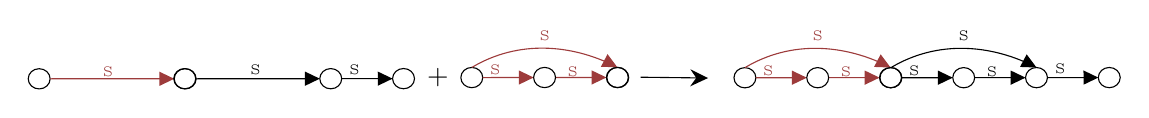
\begin{tikzpicture}[x=0.75pt,y=0.75pt,yscale=-1,xscale=1, scale=0.8]
%uncomment if require: \path (0,70); %set diagram left start at 0, and has height of 70

%Shape: Ellipse [id:dp3471974205267804] 
\draw   (1.79,33.19) .. controls (1.79,29.82) and (4.74,27.1) .. (8.38,27.1) .. controls (12.02,27.1) and (14.97,29.82) .. (14.97,33.19) .. controls (14.97,36.56) and (12.02,39.29) .. (8.38,39.29) .. controls (4.74,39.29) and (1.79,36.56) .. (1.79,33.19) -- cycle ;
%Straight Lines [id:da318667838378054] 
\draw [color={rgb, 255:red, 157; green, 59; blue, 59 }  ,draw opacity=1 ]   (14.97,33.19) -- (40.24,33.16) -- (86.71,33.19) ;
\draw [shift={(89.71,33.19)}, rotate = 180.03] [fill={rgb, 255:red, 157; green, 59; blue, 59 }  ,fill opacity=1 ][line width=0.08]  [draw opacity=0] (8.93,-4.29) -- (0,0) -- (8.93,4.29) -- cycle    ;
%Shape: Ellipse [id:dp1575171226993164] 
\draw   (89.46,33.12) .. controls (89.46,29.76) and (92.42,27.03) .. (96.06,27.03) .. controls (99.7,27.03) and (102.65,29.76) .. (102.65,33.12) .. controls (102.65,36.49) and (99.7,39.22) .. (96.06,39.22) .. controls (92.42,39.22) and (89.46,36.49) .. (89.46,33.12) -- cycle ;
%Shape: Ellipse [id:dp3728021507763205] 
\draw   (89.71,33.19) .. controls (89.71,29.82) and (92.66,27.1) .. (96.3,27.1) .. controls (99.94,27.1) and (102.9,29.82) .. (102.9,33.19) .. controls (102.9,36.56) and (99.94,39.29) .. (96.3,39.29) .. controls (92.66,39.29) and (89.71,36.56) .. (89.71,33.19) -- cycle ;
%Straight Lines [id:da5699348554411348] 
\draw [color={rgb, 255:red, 0; green, 0; blue, 0 }  ,draw opacity=1 ]   (102.9,33.19) -- (128.16,33.16) -- (174.39,33.12) ;
\draw [shift={(177.39,33.12)}, rotate = 179.95] [fill={rgb, 255:red, 0; green, 0; blue, 0 }  ,fill opacity=1 ][line width=0.08]  [draw opacity=0] (8.93,-4.29) -- (0,0) -- (8.93,4.29) -- cycle    ;
%Shape: Ellipse [id:dp3069366008412512] 
\draw   (177.39,33.12) .. controls (177.39,29.76) and (180.34,27.03) .. (183.98,27.03) .. controls (187.62,27.03) and (190.57,29.76) .. (190.57,33.12) .. controls (190.57,36.49) and (187.62,39.22) .. (183.98,39.22) .. controls (180.34,39.22) and (177.39,36.49) .. (177.39,33.12) -- cycle ;
%Straight Lines [id:da8862262788341165] 
\draw [color={rgb, 255:red, 0; green, 0; blue, 0 }  ,draw opacity=1 ]   (190.57,33.12) -- (215.83,33.09) -- (218.22,33.09) ;
\draw [shift={(221.22,33.09)}, rotate = 179.94] [fill={rgb, 255:red, 0; green, 0; blue, 0 }  ,fill opacity=1 ][line width=0.08]  [draw opacity=0] (8.93,-4.29) -- (0,0) -- (8.93,4.29) -- cycle    ;
%Shape: Ellipse [id:dp4698865456949003] 
\draw   (221.22,33.09) .. controls (221.22,29.72) and (224.17,26.99) .. (227.82,26.99) .. controls (231.46,26.99) and (234.41,29.72) .. (234.41,33.09) .. controls (234.41,36.45) and (231.46,39.18) .. (227.82,39.18) .. controls (224.17,39.18) and (221.22,36.45) .. (221.22,33.09) -- cycle ;
%Shape: Ellipse [id:dp41783743694019515] 
\draw   (262.33,32.44) .. controls (262.33,29.08) and (265.28,26.35) .. (268.92,26.35) .. controls (272.56,26.35) and (275.51,29.08) .. (275.51,32.44) .. controls (275.51,35.81) and (272.56,38.54) .. (268.92,38.54) .. controls (265.28,38.54) and (262.33,35.81) .. (262.33,32.44) -- cycle ;
%Straight Lines [id:da04365576627045986] 
\draw [color={rgb, 255:red, 157; green, 59; blue, 59 }  ,draw opacity=1 ]   (275.51,32.44) -- (300.77,32.42) -- (303.16,32.41) ;
\draw [shift={(306.16,32.41)}, rotate = 179.94] [fill={rgb, 255:red, 157; green, 59; blue, 59 }  ,fill opacity=1 ][line width=0.08]  [draw opacity=0] (8.93,-4.29) -- (0,0) -- (8.93,4.29) -- cycle    ;
%Straight Lines [id:da1625453128939066] 
\draw [color={rgb, 255:red, 157; green, 59; blue, 59 }  ,draw opacity=1 ]   (319.35,32.41) -- (344.61,32.38) -- (347,32.38) ;
\draw [shift={(350,32.38)}, rotate = 179.94] [fill={rgb, 255:red, 157; green, 59; blue, 59 }  ,fill opacity=1 ][line width=0.08]  [draw opacity=0] (8.93,-4.29) -- (0,0) -- (8.93,4.29) -- cycle    ;
%Shape: Ellipse [id:dp19846361502611898] 
\draw   (306.16,32.41) .. controls (306.16,29.04) and (309.12,26.31) .. (312.76,26.31) .. controls (316.4,26.31) and (319.35,29.04) .. (319.35,32.41) .. controls (319.35,35.78) and (316.4,38.51) .. (312.76,38.51) .. controls (309.12,38.51) and (306.16,35.78) .. (306.16,32.41) -- cycle ;
%Shape: Ellipse [id:dp7570984947626253] 
\draw   (350,32.38) .. controls (350,29.01) and (352.95,26.28) .. (356.59,26.28) .. controls (360.24,26.28) and (363.19,29.01) .. (363.19,32.38) .. controls (363.19,35.74) and (360.24,38.47) .. (356.59,38.47) .. controls (352.95,38.47) and (350,35.74) .. (350,32.38) -- cycle ;
%Curve Lines [id:da0990654981494471] 
\draw [color={rgb, 255:red, 157; green, 59; blue, 59 }  ,draw opacity=1 ]   (268.92,26.35) .. controls (297.47,9.31) and (329.26,12.88) .. (353.94,24.94) ;
\draw [shift={(356.59,26.28)}, rotate = 207.67] [fill={rgb, 255:red, 157; green, 59; blue, 59 }  ,fill opacity=1 ][line width=0.08]  [draw opacity=0] (8.93,-4.29) -- (0,0) -- (8.93,4.29) -- cycle    ;
%Shape: Ellipse [id:dp8463415335018973] 
\draw   (350.25,32.44) .. controls (350.25,29.08) and (353.2,26.35) .. (356.84,26.35) .. controls (360.48,26.35) and (363.43,29.08) .. (363.43,32.44) .. controls (363.43,35.81) and (360.48,38.54) .. (356.84,38.54) .. controls (353.2,38.54) and (350.25,35.81) .. (350.25,32.44) -- cycle ;

%Straight Lines [id:da6018407867885048] 
\draw    (370.53,32.23) -- (408.21,32.68) ;
\draw [shift={(411.21,32.72)}, rotate = 180.68] [fill={rgb, 255:red, 0; green, 0; blue, 0 }  ][line width=0.08]  [draw opacity=0] (10.72,-5.15) -- (0,0) -- (10.72,5.15) -- (7.12,0) -- cycle    ;
%Shape: Ellipse [id:dp9757220995258307] 
\draw   (426.82,32.56) .. controls (426.82,29.19) and (429.77,26.46) .. (433.41,26.46) .. controls (437.05,26.46) and (440.01,29.19) .. (440.01,32.56) .. controls (440.01,35.92) and (437.05,38.65) .. (433.41,38.65) .. controls (429.77,38.65) and (426.82,35.92) .. (426.82,32.56) -- cycle ;
%Straight Lines [id:da8161266034843465] 
\draw [color={rgb, 255:red, 157; green, 59; blue, 59 }  ,draw opacity=1 ]   (440.01,32.56) -- (465.27,32.53) -- (467.66,32.53) ;
\draw [shift={(470.66,32.52)}, rotate = 179.94] [fill={rgb, 255:red, 157; green, 59; blue, 59 }  ,fill opacity=1 ][line width=0.08]  [draw opacity=0] (8.93,-4.29) -- (0,0) -- (8.93,4.29) -- cycle    ;
%Straight Lines [id:da11562290681606402] 
\draw [color={rgb, 255:red, 157; green, 59; blue, 59 }  ,draw opacity=1 ]   (483.84,32.52) -- (509.1,32.49) -- (511.49,32.49) ;
\draw [shift={(514.49,32.49)}, rotate = 179.94] [fill={rgb, 255:red, 157; green, 59; blue, 59 }  ,fill opacity=1 ][line width=0.08]  [draw opacity=0] (8.93,-4.29) -- (0,0) -- (8.93,4.29) -- cycle    ;
%Shape: Ellipse [id:dp39996624936566727] 
\draw   (470.66,32.52) .. controls (470.66,29.16) and (473.61,26.43) .. (477.25,26.43) .. controls (480.89,26.43) and (483.84,29.16) .. (483.84,32.52) .. controls (483.84,35.89) and (480.89,38.62) .. (477.25,38.62) .. controls (473.61,38.62) and (470.66,35.89) .. (470.66,32.52) -- cycle ;
%Shape: Ellipse [id:dp5486338938310714] 
\draw   (514.49,32.49) .. controls (514.49,29.12) and (517.45,26.39) .. (521.09,26.39) .. controls (524.73,26.39) and (527.68,29.12) .. (527.68,32.49) .. controls (527.68,35.85) and (524.73,38.58) .. (521.09,38.58) .. controls (517.45,38.58) and (514.49,35.85) .. (514.49,32.49) -- cycle ;
%Curve Lines [id:da09361622227375666] 
\draw [color={rgb, 255:red, 157; green, 59; blue, 59 }  ,draw opacity=1 ]   (433.41,26.46) .. controls (461.96,9.42) and (493.76,12.99) .. (518.43,25.05) ;
\draw [shift={(521.09,26.39)}, rotate = 207.67] [fill={rgb, 255:red, 157; green, 59; blue, 59 }  ,fill opacity=1 ][line width=0.08]  [draw opacity=0] (8.93,-4.29) -- (0,0) -- (8.93,4.29) -- cycle    ;
%Shape: Ellipse [id:dp7411533555594203] 
\draw   (514.74,32.56) .. controls (514.74,29.19) and (517.69,26.46) .. (521.33,26.46) .. controls (524.97,26.46) and (527.93,29.19) .. (527.93,32.56) .. controls (527.93,35.92) and (524.97,38.65) .. (521.33,38.65) .. controls (517.69,38.65) and (514.74,35.92) .. (514.74,32.56) -- cycle ;
%Straight Lines [id:da34615602922748345] 
\draw [color={rgb, 255:red, 0; green, 0; blue, 0 }  ,draw opacity=1 ]   (527.93,32.56) -- (553.19,32.53) -- (555.58,32.53) ;
\draw [shift={(558.58,32.52)}, rotate = 179.94] [fill={rgb, 255:red, 0; green, 0; blue, 0 }  ,fill opacity=1 ][line width=0.08]  [draw opacity=0] (8.93,-4.29) -- (0,0) -- (8.93,4.29) -- cycle    ;
%Straight Lines [id:da6952718268667677] 
\draw [color={rgb, 255:red, 0; green, 0; blue, 0 }  ,draw opacity=1 ]   (571.76,32.52) -- (597.03,32.49) -- (599.42,32.49) ;
\draw [shift={(602.42,32.49)}, rotate = 179.94] [fill={rgb, 255:red, 0; green, 0; blue, 0 }  ,fill opacity=1 ][line width=0.08]  [draw opacity=0] (8.93,-4.29) -- (0,0) -- (8.93,4.29) -- cycle    ;
%Shape: Ellipse [id:dp5091308278334061] 
\draw   (558.58,32.52) .. controls (558.58,29.16) and (561.53,26.43) .. (565.17,26.43) .. controls (568.81,26.43) and (571.76,29.16) .. (571.76,32.52) .. controls (571.76,35.89) and (568.81,38.62) .. (565.17,38.62) .. controls (561.53,38.62) and (558.58,35.89) .. (558.58,32.52) -- cycle ;
%Shape: Ellipse [id:dp995169097157605] 
\draw   (602.42,32.49) .. controls (602.42,29.12) and (605.37,26.39) .. (609.01,26.39) .. controls (612.65,26.39) and (615.6,29.12) .. (615.6,32.49) .. controls (615.6,35.85) and (612.65,38.58) .. (609.01,38.58) .. controls (605.37,38.58) and (602.42,35.85) .. (602.42,32.49) -- cycle ;
%Curve Lines [id:da541208105388246] 
\draw [color={rgb, 255:red, 0; green, 0; blue, 0 }  ,draw opacity=1 ]   (521.33,26.46) .. controls (549.88,9.42) and (581.68,12.99) .. (606.35,25.05) ;
\draw [shift={(609.01,26.39)}, rotate = 207.67] [fill={rgb, 255:red, 0; green, 0; blue, 0 }  ,fill opacity=1 ][line width=0.08]  [draw opacity=0] (8.93,-4.29) -- (0,0) -- (8.93,4.29) -- cycle    ;
%Straight Lines [id:da001396932560887465] 
\draw [color={rgb, 255:red, 0; green, 0; blue, 0 }  ,draw opacity=1 ]   (615.6,32.49) -- (640.86,32.46) -- (643.25,32.46) ;
\draw [shift={(646.25,32.45)}, rotate = 179.94] [fill={rgb, 255:red, 0; green, 0; blue, 0 }  ,fill opacity=1 ][line width=0.08]  [draw opacity=0] (8.93,-4.29) -- (0,0) -- (8.93,4.29) -- cycle    ;
%Shape: Ellipse [id:dp8196920302499935] 
\draw   (646.25,32.45) .. controls (646.25,29.09) and (649.21,26.36) .. (652.85,26.36) .. controls (656.49,26.36) and (659.44,29.09) .. (659.44,32.45) .. controls (659.44,35.82) and (656.49,38.55) .. (652.85,38.55) .. controls (649.21,38.55) and (646.25,35.82) .. (646.25,32.45) -- cycle ;

% Text Node
\draw (45.23,24.35) node [anchor=north west][inner sep=0.75pt]  [font=\tiny,color={rgb, 255:red, 157; green, 59; blue, 59 }  ,opacity=1 ] [align=left] {S};
% Text Node
\draw (133.96,23.61) node [anchor=north west][inner sep=0.75pt]  [font=\tiny,color={rgb, 255:red, 0; green, 0; blue, 0 }  ,opacity=1 ] [align=left] {S};
% Text Node
\draw (193.65,23.61) node [anchor=north west][inner sep=0.75pt]  [font=\tiny,color={rgb, 255:red, 0; green, 0; blue, 0 }  ,opacity=1 ] [align=left] {S};
% Text Node
\draw (278.34,23.61) node [anchor=north west][inner sep=0.75pt]  [font=\tiny,color={rgb, 255:red, 157; green, 59; blue, 59 }  ,opacity=1 ] [align=left] {S};
% Text Node
\draw (325.12,24.35) node [anchor=north west][inner sep=0.75pt]  [font=\tiny,color={rgb, 255:red, 157; green, 59; blue, 59 }  ,opacity=1 ] [align=left] {S};
% Text Node
\draw (308.19,2.73) node [anchor=north west][inner sep=0.75pt]  [font=\tiny,color={rgb, 255:red, 157; green, 59; blue, 59 }  ,opacity=1 ] [align=left] {S};
% Text Node
\draw (240.46,25.19) node [anchor=north west][inner sep=0.75pt]   [align=left] {+};
% Text Node
\draw (442.83,23.72) node [anchor=north west][inner sep=0.75pt]  [font=\tiny,color={rgb, 255:red, 157; green, 59; blue, 59 }  ,opacity=1 ] [align=left] {S};
% Text Node
\draw (489.62,24.47) node [anchor=north west][inner sep=0.75pt]  [font=\tiny,color={rgb, 255:red, 157; green, 59; blue, 59 }  ,opacity=1 ] [align=left] {S};
% Text Node
\draw (472.68,2.84) node [anchor=north west][inner sep=0.75pt]  [font=\tiny,color={rgb, 255:red, 157; green, 59; blue, 59 }  ,opacity=1 ] [align=left] {S};
% Text Node
\draw (530.76,23.72) node [anchor=north west][inner sep=0.75pt]  [font=\tiny,color={rgb, 255:red, 0; green, 0; blue, 0 }  ,opacity=1 ] [align=left] {S};
% Text Node
\draw (577.54,24.47) node [anchor=north west][inner sep=0.75pt]  [font=\tiny,color={rgb, 255:red, 0; green, 0; blue, 0 }  ,opacity=1 ] [align=left] {S};
% Text Node
\draw (560.6,2.84) node [anchor=north west][inner sep=0.75pt]  [font=\tiny,color={rgb, 255:red, 0; green, 0; blue, 0 }  ,opacity=1 ] [align=left] {S};
% Text Node
\draw (618.68,22.97) node [anchor=north west][inner sep=0.75pt]  [font=\tiny,color={rgb, 255:red, 0; green, 0; blue, 0 }  ,opacity=1 ] [align=left] {S};


\end{tikzpicture}

\end{center}
Functional view: \newline 
\hspace*{.05\textwidth} Sequential(\textcolor[HTML]{9D3B3B}{S},S,S) \hspace*{.11\textwidth}  + \textcolor[HTML]{9D3B3B}{Residual(S,S,S)} \hspace*{.01\textwidth} $\longrightarrow$ \hspace*{.01\textwidth}Sequential(\textcolor[HTML]{9D3B3B}{Residual(S,S,S)},S,S,S)

\end{frame}

\begin{frame}{Hierarchical NAS-Bench-201}
Newer Search Space \liturl{Schrodi et al. 2023}{https://proceedings.neurips.cc/paper_files/paper/2023/file/4869f3f967dfe954439408dd92c50ee1-Paper-Conference.pdf}

\begin{equation*}\label{eq:hnb201}
    \resizebox{\linewidth}{!}{%
    $\begin{aligned}
         \mathrm{D2}~::=~&~\textcolor{myblue}{\texttt{Sequential3}(\mathrm{D1},\;\mathrm{D1},\;\mathrm{D0})}~~|~~\textcolor{myblue}{\texttt{Sequential3}(\mathrm{D0},\;\mathrm{D1},\;\mathrm{D1})}~~|~~\textcolor{myblue}{\texttt{Sequential4}(\mathrm{D1},\;\mathrm{D1},\;\mathrm{D0},\;\mathrm{D0})}\\
         \mathrm{D1}~::=~&~\textcolor{myblue}{\texttt{Sequential3}(\mathrm{C},\;\mathrm{C},\;\mathrm{D})}~~|~~\textcolor{myblue}{\texttt{Sequential4}(\mathrm{C},\;\mathrm{C},\;\mathrm{C},\;\mathrm{D})}~~|~~\textcolor{myblue}{\texttt{Residual3}(\mathrm{C},\;\mathrm{C},\;\mathrm{D},\;\mathrm{D})}\\
         \mathrm{D0}~::=~&~\textcolor{myblue}{\texttt{Sequential3}(\mathrm{C},\;\mathrm{C},\;\mathrm{CL})}~~|~~\textcolor{myblue}{\texttt{Sequential4}(\mathrm{C},\;\mathrm{C},\;\mathrm{C},\;\mathrm{CL})}~~|~~\textcolor{myblue}{\texttt{Residual3}(\mathrm{C},\;\mathrm{C},\;\mathrm{CL},\;\mathrm{CL})}\\
         \mathrm{D}~::=~&~\textcolor{myblue}{\texttt{Sequential2}( \mathrm{CL},\;\texttt{down})}~~|~~\textcolor{myblue}{\texttt{Sequential3}(\mathrm{CL},\;\mathrm{CL},\;\texttt{down})}~~|~~\textcolor{myblue}{\texttt{Residual2}(\mathrm{CL},\;\texttt{down},\;\texttt{down})}\\
         \mathrm{C}~::=~&~\textcolor{myblue}{\texttt{Sequential2}(\mathrm{CL},~ \mathrm{CL})}~~|~~\textcolor{myblue}{\texttt{Sequential3}(\mathrm{CL},\;\mathrm{CL},\;\mathrm{CL})}~~|~~\textcolor{myblue}{\texttt{Residual2}(\mathrm{CL},\;\mathrm{CL},\;\mathrm{CL})}\\
         \mathrm{CL}~::=~&~\textcolor{myred}{\texttt{Cell}(\mathrm{OP},\;\mathrm{OP},\;\mathrm{OP},\;\mathrm{OP},\;\mathrm{OP},\;\mathrm{OP})}\\
         \mathrm{OP}~::=~&~\textcolor{myred}{\texttt{zero}}~~|~~\textcolor{myred}{\texttt{id}}~~|~~\textcolor{myred}{\mathrm{CONVBLOCK}}~~|~~\textcolor{myred}{\texttt{avg\_pool}}\\
         \mathrm{CONVBLOCK}~::=~&~\textcolor{myred}{\texttt{Sequential3}(\mathrm{ACT},~ \mathrm{CONV},~ \mathrm{NORM})}\\
         \mathrm{ACT}~::=~&~\textcolor{myred}{\texttt{relu}}~~|~~\textcolor{myyellow}{\texttt{hardswish}}~~|~~\textcolor{myyellow}{\texttt{mish}}\\
         \mathrm{CONV}~::=~&~\textcolor{myred}{\texttt{conv1x1}}~~|~~\textcolor{myred}{\texttt{conv3x3}}~~|~~\textcolor{myyellow}{\texttt{dconv3x3}}\\
         \mathrm{NORM}~::=~&~\textcolor{myred}{\texttt{batch}}~~|~~\textcolor{myyellow}{\texttt{instance}}~~|~~\textcolor{myyellow}{\texttt{layer}} \qquad .
    \end{aligned}$%
    }
\end{equation*}
    
\end{frame}

\begin{frame}{Hierarchical NAS-Bench-201}
\begin{itemize}
\item This search space provides us with $10^{446}$ different architectures, however only CNNs
\item einspace \liturl{Ericsson et al. 2024}{https://openreview.net/pdf?id=qf1ncViBr5} is also based on CFGs
\item Unifies different network families, including CNNs, Transformers and MLP-only, as well as hybrid versions.
\end{itemize}

\end{frame}

\begin{frame}{einspace \liturl{Ericsson et al. 2024}{https://openreview.net/pdf?id=qf1ncViBr5}}
Fundamental Operations categorized in four groups
\begin{columns}
\begin{column}{0.65\textwidth}
   \begin{itemize}
       \item \textcolor{fig2_yellow}{Branching}: \textit{one-to-many} functions that split or clone tensors (e.g., clone)
       \item \textcolor{fig2_purple}{Aggregation}: \textit{many-to-one} functions that merge multiple tensors into one (e.g., matrix mulitplication, addition, concatenation)
       \item \textcolor{fig2_green}{Routing}: \textit{one-to-one} functions that change the shape or the order within a tensor (e.g., permute)
       \item \textcolor{fig2_blue}{Computation}: \textbf{one-to-one} functions that alter the information of the tensor (e.g., linear, activation, positional encoding)
       \end{itemize}
\end{column}
    
\begin{column}{0.35\textwidth}
\begin{figure}
    \centering
    
\includegraphics[width=0.5\linewidth]{07_NAS/images/07/einspace_example_modules.pdf}
    \caption{Macro Structures from \liturl{Ericsson et al. 2024}{https://openreview.net/pdf?id=qf1ncViBr5} }
    \label{fig:placeholder}
\end{figure}
\end{column}

\end{columns}

\end{frame}

\begin{frame}{einspace \liturl{Ericsson et al. 2024}{https://openreview.net/pdf?id=qf1ncViBr5}}

\begin{tcolorbox}[
    colback=white,
    colframe=black!60,
    sharpish corners=all,
    boxsep=0em,
    left=1em,
    top=0em,
    % fuzzy shadow={0mm}{0pt}{-1pt}{0.2mm}{black!30!white},
    % enhanced,
]
\begin{align*}
    \texttt{S} \quad &\rightarrow \quad \texttt{M} \quad \texttt{M} \quad | \quad \texttt{B} \quad \texttt{M} \quad \texttt{A} \quad | \quad \texttt{P} \quad \texttt{M} \quad \texttt{R}, \quad \\
    \texttt{M} \quad &\rightarrow \quad \texttt{M} \quad \texttt{M} \quad | \quad \texttt{B} \quad \texttt{M} \quad \texttt{A} \quad | \quad \texttt{P} \quad \texttt{M} \quad \texttt{R} \quad | \quad \texttt{C}, \\
    \texttt{\textcolor{fig2_yellow}{B}} \quad &\rightarrow \quad \texttt{\textcolor{fig2_yellow}{clone}} \quad | \quad \texttt{\textcolor{fig2_yellow}{group}}, \\
    \texttt{\textcolor{fig2_purple}{A}} \quad &\rightarrow \quad \texttt{\textcolor{fig2_purple}{matmul}} \quad | \quad \texttt{\textcolor{fig2_purple}{add}} \quad | \quad \texttt{\textcolor{fig2_purple}{concat}}, \quad \\
    \texttt{\textcolor{fig2_green}{P}} \quad &\rightarrow \quad \texttt{\textcolor{fig2_green}{identity}} \quad | \quad \texttt{\textcolor{fig2_green}{im2col}} \quad | \quad \texttt{\textcolor{fig2_green}{permute}}, \\
    \texttt{\textcolor{fig2_green}{R}} \quad &\rightarrow \quad \texttt{\textcolor{fig2_green}{identity}} \quad | \quad \texttt{\textcolor{fig2_green}{col2im}} \quad | \quad \texttt{\textcolor{fig2_green}{permute}}, \\
    \texttt{\textcolor{fig2_blue}{C}} \quad &\rightarrow \quad \texttt{\textcolor{fig2_blue}{identity}} \quad | \quad \texttt{\textcolor{fig2_blue}{linear}} \quad | \quad \texttt{\textcolor{fig2_blue}{norm}} \quad | \quad \texttt{\textcolor{fig2_blue}{relu}} \quad | \quad \texttt{\textcolor{fig2_blue}{softmax}} \quad | \quad \texttt{\textcolor{fig2_blue}{pos-enc}}. \quad
\end{align*}
\end{tcolorbox}
This CFG defines einspace, with uppercase symbols being non-terminals and lowercase being terminals. The colours refer to the fundamental operations group.
\end{frame}

\begin{frame}{Summary}
    
Most important insights from this video:

\begin{enumerate}
    \item Newer NAS approaches aim for expressive search spaces
    \item This allows for the possibility of finding novel networks
    \item Allows for better studies and improvements of the actual search
\end{enumerate}
\end{frame}



\end{document}